\section{Softwarearkitektur}
Dette afsnit beskriver softwarearkitekturen. For at give det fornødne overblik over softwarearkitekturen i vores system, har vi valgt at inkludere en overordnet domænemodel, en domænemodel for software samt et tomt klassediagram uden attributter og metoder. I afsnittet design findes sekvensdiagram og klassediagram for UC1. Diagrammer er med til at danne grundlaget for software designprocessen. Ved at man bryder systemet ned i mindre dele, giver det tilmed også et overblik over hvad der skal foregå i systemet, og dette gør det nemmere at finde frem til designløsninger. Nedenstående figur den overordnede domænemodel, som giver et overblik og hele systemet. 

\subsection{Overordnet domænemodel}
	\begin{figure}[h!]
	\centering
	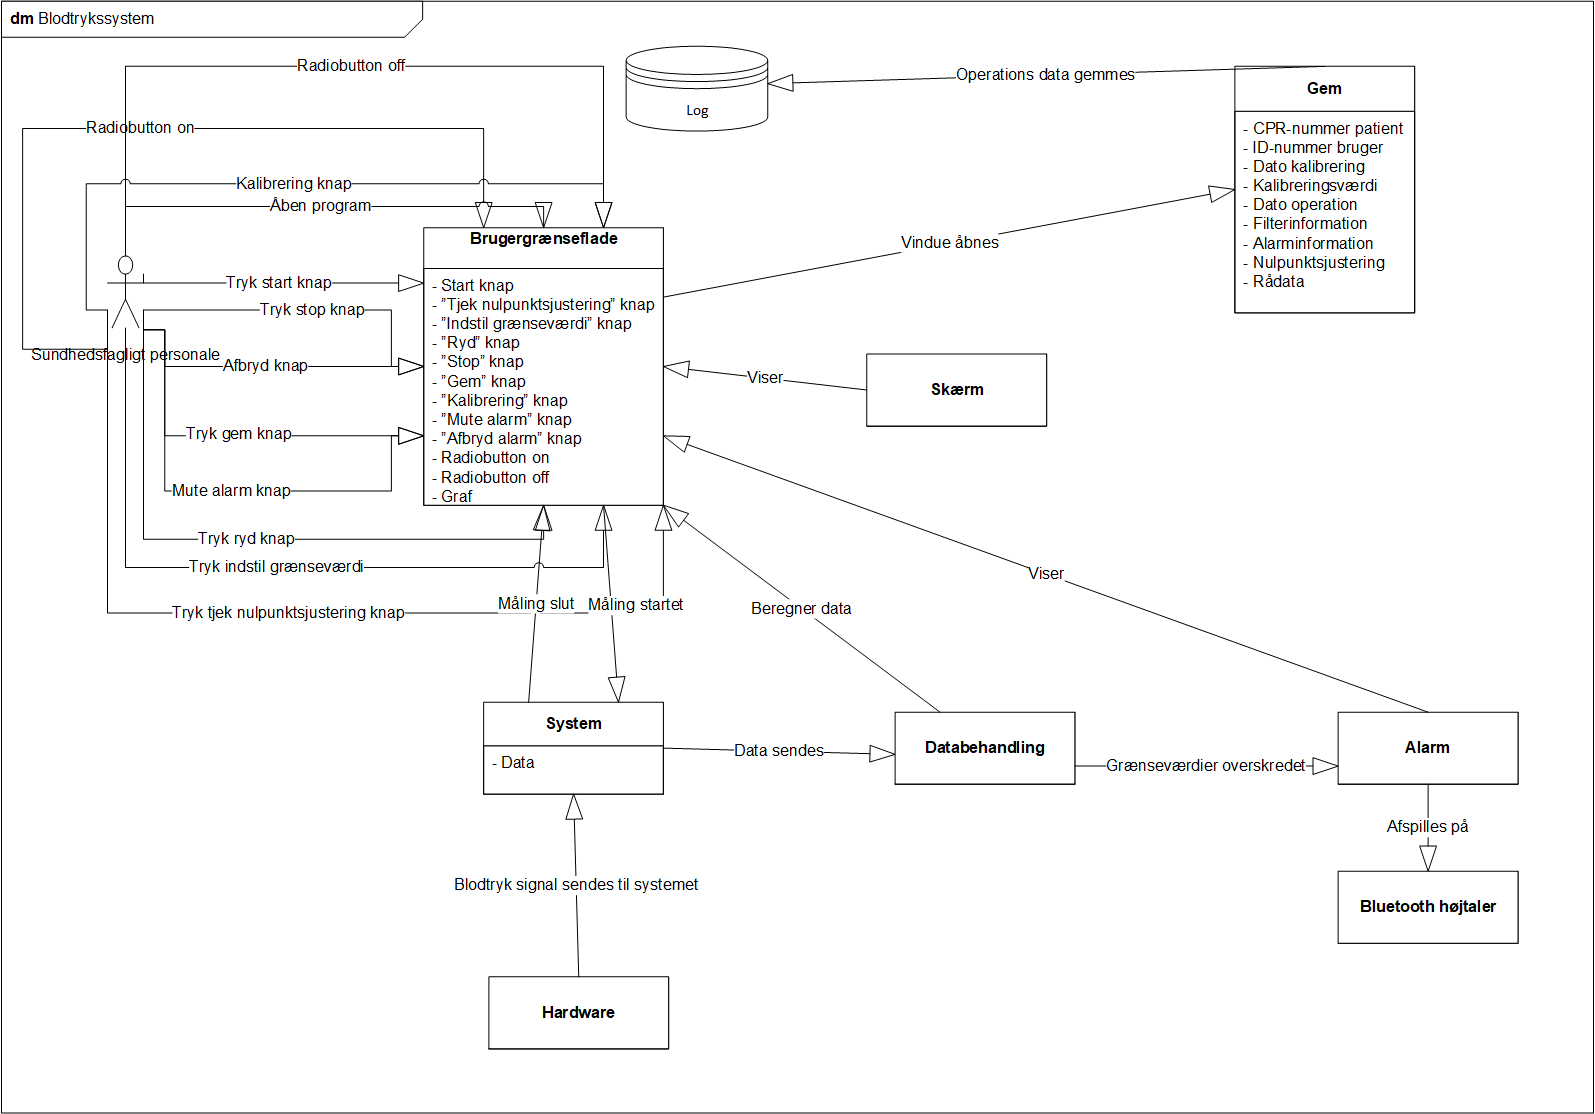
\includegraphics[width=1\linewidth]{Arkitektur_og_design/Softwarearkitektur/overordnetdomain}
	\label{fig:overordnetdomain}
	\caption{Overordnet domænemodel}
\end{figure}

Ovenstående figur \vref{fig:overordnetdomain} illustrerer den overordnede domænemodel, som viser både hardware og software. Domæneklassrne fandt vi efter en navneords analyse af vores fully dressed use cases, hvor vi fandt frem til brugergrænseflade, sundhedsfagligt personale, log, skærm, gem, system, databehandling, alarm og bluetooth højtaler.  Log domænet er en tekstfil, hvor oplysninger fra operationen gemmes i.

\subsection{Domænemodel for software}
  
Ud fra vores kendskab til domænet, har vi lavet en software-domænemodel, hvor vi får et overblik over, hvilke domæneklasser vores software skal indeholde. 

\clearpage

\begin{figure}[h!]
	\centering
	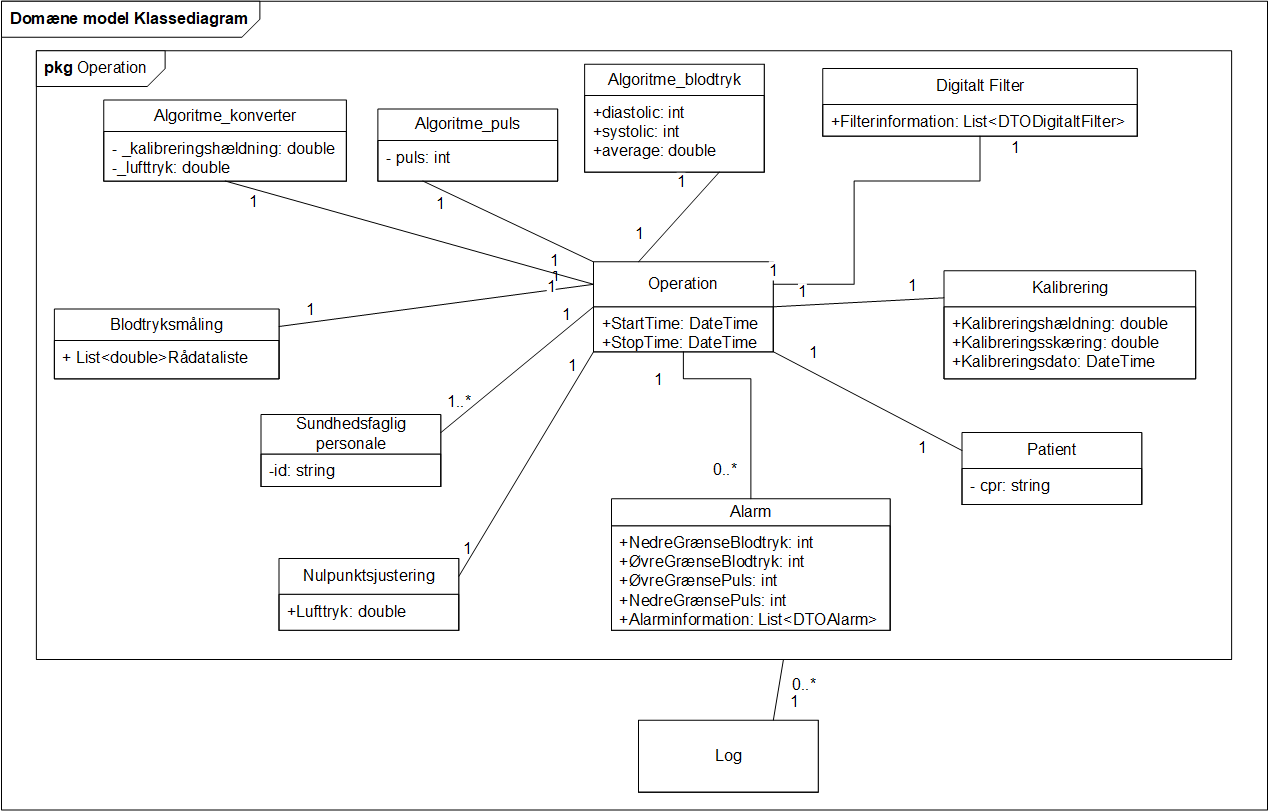
\includegraphics[width=1\linewidth]{Arkitektur_og_design/Softwarearkitektur/classdomain}
	\label{fig:classdomain}
	\caption{Domænemodel for software}
\end{figure}

Ovenstående figur \vref{fig:classdomain} viser systemets domæne for softwaren og hvilke klasser dette er bestående af.  Herudover viser den relationen mellem de forskellige domæneklasser og operationen. For eksempel kan der ved 1 operation være 0 til mange alarmer, som er illustreret ved "0..*". Modellen viser også en oversigt over klassernes tilhørende attributter og typerne af disse. Typerne har vi rationaliseret os frem til ved viden om at vores målinger vil være decimaltal (doubles), vores beregner vil vi gerne have vist i heltal (int), id og cpr er hensigtmæssigt at gemme som en string, og så vi nogle start- og stoptidspunkter som er oplagte at lave som DateTime. 

Ud fra vores use cases er vi kommet frem til, at ovenstående domæneklasser kan beskrive vores domæne tilstrækkeligt. Det gjorde vi, som tidligere nævnt, ved at lave en navnordsanalyse af vores fullydressed use cases. Ud fra denne fandt vi domæneklasserne: sundhedsfagligt personale, nulpunktsjustering, patient, alarm, kalibrering, digitalt filter, blodtryksmåling samt log. Ud fra disse gav det mening at samle det hele under klassen operation, som er vores brugssituation. Vi indså, at vi manglede klasser for vores databehandling. Dette delte vi op i tre klasser. En til pulsalgoritme, en til blodstryksalgoritme og en klasse til at konvertere fra volt til mmHg. 

Dernæst lavede vi et overordnet tomt klassediagram, som er udformet på baggrund af vores use cases. Klasserne fra software domænemodellen er en del af vores Model package, som indeholder domæneklasser og dtoklasser. 

\clearpage

\begin{figure}[h!]
	\centering
	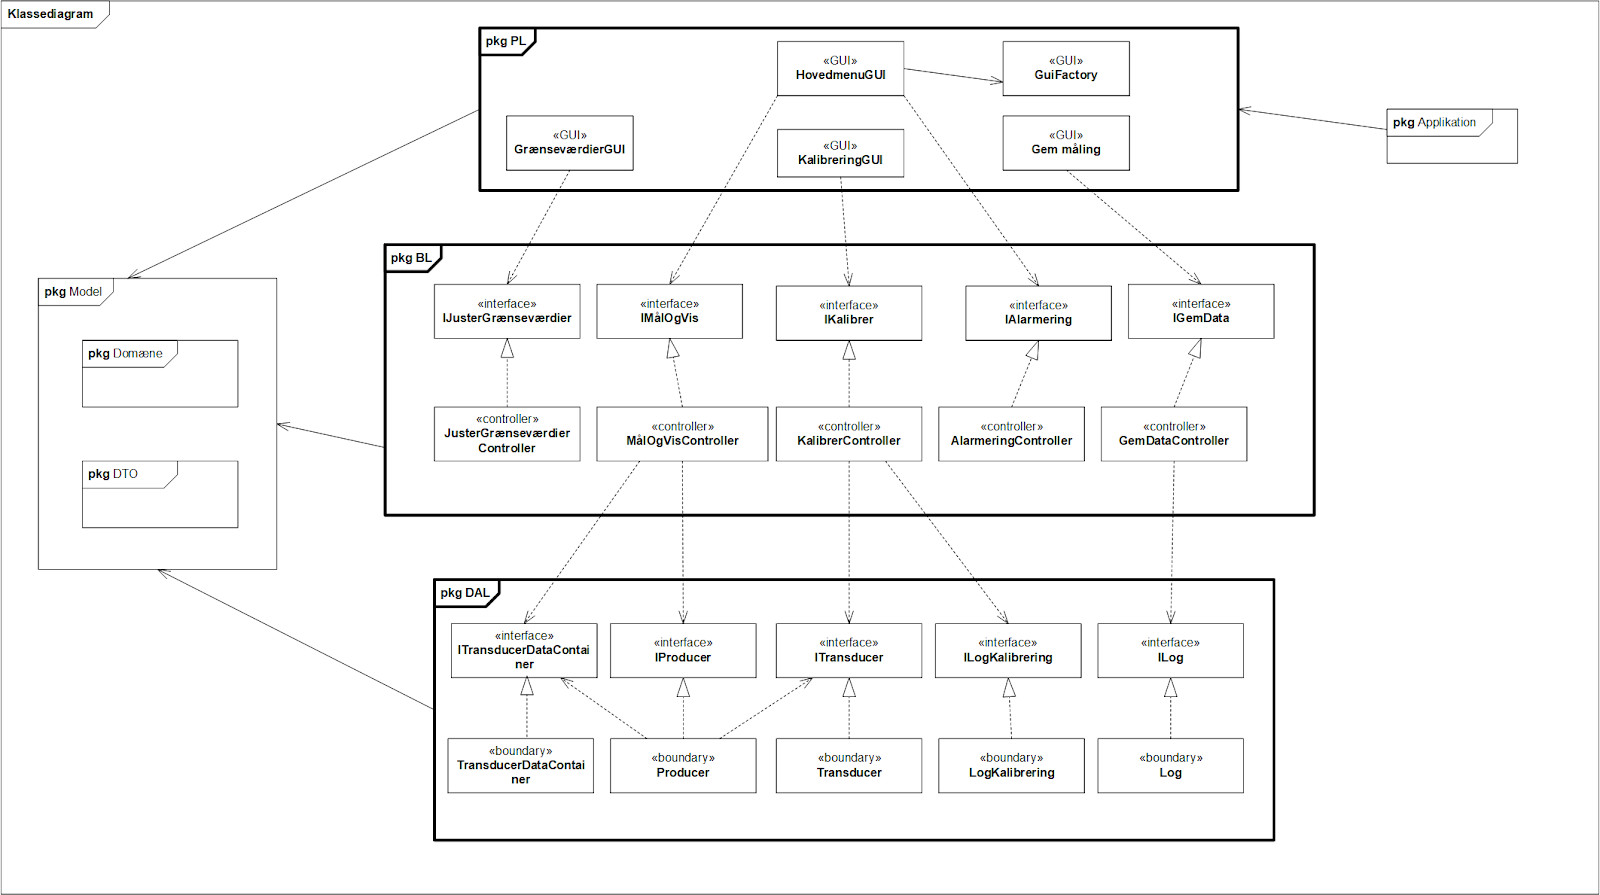
\includegraphics[width=1\linewidth]{Arkitektur_og_design/Softwarearkitektur/tomclass}
	\label{fig:tomclass}
	\caption{Klassediagram uden attributter og metoder}
\end{figure}

Klassediagrammet på figur \vref{fig:tomclass} viser opbygningen af softwaren. Vi har valgt at bygge vores system op efter trelagsmodellen, med præsentationslag (PL), businesslag (BL) og datalag (DAL). Dette er en god opbygning af et større system, som skal indhente, behandle og vise data.
